% !TEX root = ../main.tex

\section{Results}

Our grounded theory analysis of industry documents resulted in the creation of 25 technical primitives, 18 technical properties, 11 normative properties, 11 capabilities, and 19 use case categories.
The technical primitives, technical properties, normative properties, and capabilities are shown in Figure~\ref{fig:grounded-theory-main} and the use case categories are shown in Figure~\ref{fig:grounded-theory-apps}.
In both Figures, the various items are connected with directional arrows; these arrows roughly represent a dependency relationship with the item being pointed to relying on the item that is being pointed from, though in most cases it is the relationship rather than the directionality of the arrow that is most important.

In this section, we describe how our results provide answers to three of our questions:  (1) what exactly is Blockchain technology, (2) what capabilities does it provide, (3) how does it compare to other approaches (e.g., distributed databases).

\subsection{What is Blockchain Technology?}
Our description of Blockchain technology is based on the technical primitives and properties identified during our analysis.
This analysis revealed three key components to Blockchain technology: shared governance and operation, a cryptographically-authenticated append-only ledger, and replication.
By themselves, these components are nothing new, but used together they form what is known as Blockchain technology or Blockchain for short.

\subsubsection{Shared Governance and Operation}
At the heart of Blockchain technology is the principle of shared governance and operation.
Either of these properties is common by itself; for example, having multiple parties govern how a system should function, but then relying on trusted third-parties to operate and maintain the system.
Alternatively, the literature is rife with well-defined systems that don't need ongoing governance, but require multiple parties to actually operate and maintain the system.

Blockchain is distinct, though, not necessarily unique, in that it requires a core set of participants---referred to hereafter as \emph{miners}---who are responsible for both deciding how the system should function (i.e., shared governance) and then for operating that system.
This type of shared governance is appropriate when miners are not able to sufficiently trust each other or a third-party to faithfully govern and operate a system.
By participating in all aspects of governance and operation, each miner can be assured that the system is operating as intended.
Even if some of the miners are compromised, the other miners retain the ability to detect malicious actions by the compromised miner and to prevent it from affecting the system.
In this regard, Blockchain technology provides \emph{diffused trust} wherein it is not individual miners but rather the collective of all miners that is trusted.\footnote{This property has incorrectly been called ``trustlessness''. This is incorrect as trust still exists, it has just been diffused amongst multiple parties.} 

This shared governance and operation is executed using one or more \emph{consensus protocols} (e.g., proof-of-work~\cite{DN93,back1997partial,NakamotoS8}, byzantine fault tolerance~\cite{castro1999practical}).
The first consensus protocol is used by miners to determine what operations---known as \emph{transactions}---will be allowed to alter the state of the Blockchain system.
The second consensus protocol is used by miners to determine the rules that will be used to validate transactions in the first consensus protocol.
While governance could be conducted and recorded in transactions, removing the need for the second consensus protocol, we are not aware of any Blockchain systems that do so.

In practice, this second consensus protocol is usually an informal process in which changes to the first consensus protocol are discussed in a secondary channel (e.g., on an Internet discussion board), and consensus is established based on the number of miners that adopt the modified rules.
This ad-hoc consensus mechanisms means that it is possible for a Blockchain system to split, with one system being run by the set of miners continuing to operate using the original rules, and the other system being run by set of miners using the new rules.
Such a split is known as a \emph{fork}.
Often these forks are temporary, with miners either choosing to all adopt the new rules or to return to the original rules, but it is possible for a fork to result in the permanent creation of two non-interoperable Blockchain systems (e.g., Bitcoin Classic and Bitcoin Cash).

In Blockchain systems that use a majority-voting consensus mechanism for transaction validation, there is a concept of soft- and hard-forks.
In a soft fork, transactions that validate with the modified rules will also validate with the original rules, but transactions that validate with the original rules might not validate with the modified rules.
In a hard fork, transactions that validate with the modified rules will not necessarily validate with the original rules.
The benefit of a soft fork is that both sets of miners can continue participating in the first consensus protocol, with transactions following the modified rules always being accepted and the transactions following the original rules only being accepted if their is a majority of miners who still use the original rules.
While a soft-fork is not a permanent situation, it can provide time for miners to slowly adopt the modified protocol while allowing both sets of miners to operate on the same data.

Blockchain systems can be separated based on how they select who can act as miner:

\begin{itemize}
	\item \emph{Open governance.}
	Any party that is willing to participate in the consensus protocol is allowed to do so.
	As such, these systems are susceptible to Sybil attacks and it is necessary for them to use consensus protocols that rely on miners  proving ownership of some resource rather than relying on the miner's identity.
	Proof-of-work (demonstrating ownership of computing resources) and proof-of-stake (demonstrating ownership of digital assets stored by the Blockchain system) are the most common methods~\cite{Bano17,garay2018consensus}.
	
	\item \emph{Consortium governance.}
	Only approved miners that can attest to their identity are allowed to participate in the consensus protocol.
	The initial set of approved miners is defined at system initialization.
	If membership in the group of miners remains static over the lifetime of the system it is known as a \emph{static consortium}.
	Alternatively, in an \emph{agile consortium} miners change over time, either based on the rules of the system (e.g., random selection) or through consensus by the existing miners.
	Because miners in a consortium have a known identity they can use Byzantine Fault Tolerant consensus protocols, which do not require the resource expenditure of the Sybil-resistant protocols used in open governance-based systems~\cite{Bano17,garay2018consensus}.		
\end{itemize}

For each type of governance, there is a need to incentivize correct participant behavior.
The first type of incentive is an \emph{intrinsic incentive}---i.e., miners maintain the system faithfully because they derive value from using it.
Next, \emph{on-chain incentives} are when the Blockchain system provides direct benefits to miners for faithfully executing the system (e.g., minting currency and giving it to the miners).
Finally, \emph{off-chain incentives} are any incentive that is not managed by the Blockchain system---for example, contractual obligations or reputation.
Importantly, off-chain incentives only apply to consortium governance as they inherently rely on knowing the identity of the miners.

\subsubsection{Append-Only Ledger}
While a Blockchain system might store its current state for convenience and performance, this is not actually a requirement in Blockchain technology.
Instead, the key data structure in Blockchain technology is a cryptographically authenticated data structure~\cite{tamassia2003authenticated} that stores a history of all the transactions that have been approved by the miners.
This \emph{ledger} provides full system provenance and allows for miners or other outside parties to audit the system.
In Bitcoin, this ledger is colloquially referred to as the ``blockchain'', but we avoid that term as it unnecessarily confusing to try and discuss both Blockchain (big-B) technology and the blockchain (little-b) data structure.

The first item in the append-only ledger is known as the \emph{genesis block}.
The genesis block is responsible for identifying the initial parameters for the system.
Whenever a new transaction is approved by the miners, it will be added to the ledger and cryptographically linked to one or more preceding transactions (or the genesis block for the first transaction)~\cite{bayer1993improving,haber1990time,haber1997secure}---for example, by signing a combination of the latest transaction and a hash of the transactions it is linked to.
The resulting data structure can be either linear (e.g., Bitcoin's hash chain) or branching (e.g., Merkle tree, directed acyclic graph).
Regardless of the underlying structure it is critical that all transactions are strictly ordered and that this ordering never changes.

Transactions stored in the append-only ledger can contain any data allowed by the consensus protocol, but in practice transactions are usually concerned with \emph{tokens}.
Tokens represent a resource that is either on-chain (e.g., cryptocurrency, a document) or off-chain (e.g., a diamond, a file stored in the cloud) and are used to track that resource within the Blockchain system.
For off-chain assets, there needs to be the ability to \emph{staple} the on-chain token to the off-chain assets.
While there have been a variety of proposals for doing this (e.g., etching the token's Id onto the physical items), effective stapling remains an open research challenge.

\subsubsection{Replication}
The append-only ledger is replicated amongst all miners and is essential for several reasons.
First, during the consensus protocol it is necessary for miners to be aware of previous transactions that might invalidate the transaction being considered for approval.
Second, it removes a single point of failure preventing the loss of data at one site from impacting the system.
Third, it protects against malicious attempts to modify the append-only ledger. Without replication it would still be possible to detect that data had been corrupted, but without the replication there is no guarantee that it could be restored.

Some Blockchain systems try to limit the amount of data any given miners need to replicate by segmenting the data and assigning miners to handle governance and operations for only a subset of the system.
This is known as \emph{sharding}, with individual segments of the data known as \emph{shards}.
Sharding can drastically reduce the amount of data that miners need to store while also increasing the performance of the consensus protocols which often scale based on the number of miners.
Still, sharding comes with the drawback that miners are no longer able to audit the system as a whole.
Additionally, by reducing the number of miners responsible for any given transaction, it also reduces the number of miners an adversary would need to compromise to attack a given shard.

\subsection{Blockchain Technology's Capabilities}
Blockchain technology assembles its various technical primitive and properties to provide several key capabilities.

\subsubsection{Provenance and Auditability}
Blockchain systems provide a complete history of all transactions that were approved by the consensus process (i.e., full-system provenance).
While failed transactions are not normally written to the ledger, they could be if needed by the system for auditability.
This information can be used by the miners to audit the system and ensure that it has always followed the appropriate rules.
Additionally, this information can be used by non-miners to verify that the system is being governed and operated correctly.

If transactions are used to store information regarding digital or real-world resources (using tokens), then the provenance information for the Blockchain system can also be used to provide audit information for those resources.
This can be used to track physical, off-chain assets (e.g., supply chain management, tracking diamonds), digital, off-chain assets (e.g., copyrighted digital media), or digital, on-chain assets (e.g., cryptocurrencies, files).
 
\subsubsection{Access Control and Anonymity}
Whether a user of a Blockchain system is able to create, update, or delete a token is based on permissions defined by the miners.
While these permissions could be tracked using traditional access control paradigms, most often they are regulated cryptographically.
In this paradigm, when a token is created it is also associated with a public key.
The ability to update or delete this token is then granted to any users that can prove knowledge of the corresponding private key (e.g., by generating a signature that validates with the public key attached to the token).
Ownership of the token can be transferred or shared by associating it with a new public key.

The biggest challenge towards key-based ownership of tokens is the need to manage a public key infrastructure (PKI).
This is both a hassle technically~\cite{CT} as well as for users~\cite{ruoti2015johnny,barber2012bitter}.
One advantage of having key-based, not user-based ownership of tokens is that it allows for anonymity in the ownership and use of tokens.
Still, this requires careful attention in the system design to use appropriate cryptographic techniques (e.g., zero-knowledge proofs, mix networks, secure multi-party computation) to avoid linking real-world individuals to their keys and actions.
 
\subsubsection{Resilience}
The use of a consensus protocol and data protection provides significant resilience to Blockchain systems.
Most importantly, the compromise of a single miner, or even a small number of miners, will not impact the functionality of the system.
If the compromised miner attempts to include fraudulent transactions, these transactions will be detected and rejected by the other consensus partners.
These partners can even alert the compromised party that they have been acting oddly and might be compromised.

If a miner's data is lost or corrupted---either accidentally or maliciously---that miner will be able to restore their copy of data by replicating it from other miners.
In such cases, the miner recovering from data loss is responsible for verifying that the genesis block is correct and that each successive transaction follows the established rules, including his participation as a miner.
In this way, rebuilding a data store represents diffused trust in the system and not individual trust in any given miner.

\subsubsection{Smart Contracts}
Blockchain tokens can also represent and store executable functions known as \emph{smart contracts}.
These smart contracts can be executed automatically in response to a function call in later transactions, with both the inputs and outputs of the function recorded within the calling transaction.
The smart contracts themselves are executed by the miners with outputs being verified through the consensus protocol.
The computational power of these scripts is determined is the system's rules, ranging from supporting only basic functionality (e.g., verifying a signature in Bitcoin) to providing Turing-complete functionality (e.g., Etherium).

Smart contracts benefit from Blockchain technology's other capabilities (e.g., shared operation, auditability, and resilience).
For example, multiple miners execute and verify the output of a smart contract helps ensure that an adversary is unable to tamper with the result of a function.
Similarly, the ability to audit inputs and outputs can be used to attribute incorrect usage of a smart contract.
Still, smart contracts suffer from problems common to all programs (e.g., bugs, security flaws, complexity, non-termination) and an failure to recognize this reality can lead to disastrous consequences.\footnote{This is best exemplified by the debate over ``code is law'' and the DAO attack: \url{https://www.coindesk.com/understanding-dao-hack-journalists/}.}

\subsection{Relationship to other distributed systems}
Blockchain technology fits within the broader family of distributed systems.
At the highest level, Blockchain technology is a type of decentralized database.
To help readers situate Blockchain technology within this greater ecosystem we have created a taxonomy and a flowchart based on that taxonomy (see Figure~\ref{fig:blockchainFlowchart}).

\begin{figure*}
	\centering
	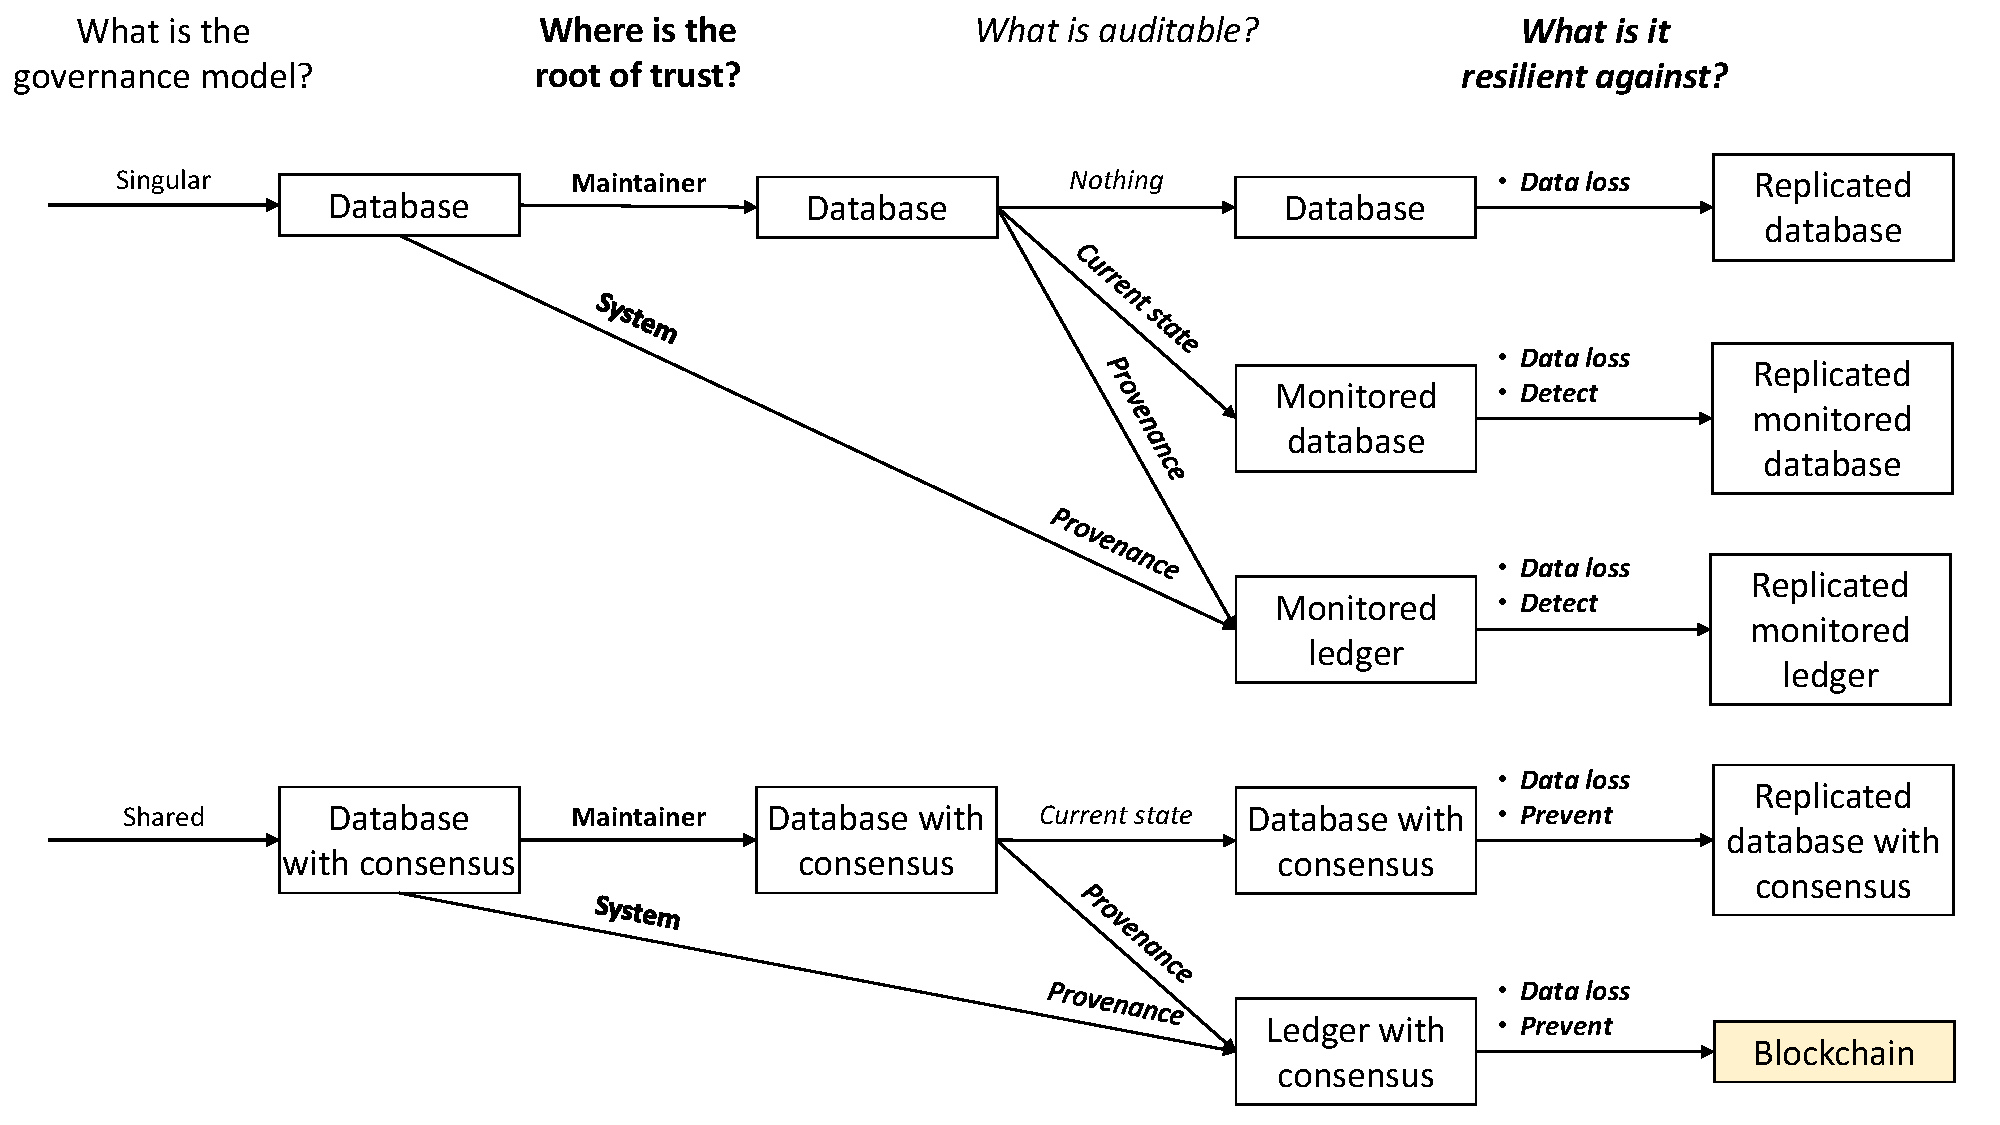
\includegraphics[width=\textwidth]{figures/BlockchainFlowchart}
	\caption{Comparing decentralized databases. Blockchain is highlighted in the bottom right corner.}
	\label{fig:blockchainFlowchart}
\end{figure*}

The first property in our taxonomy considers who has the authority to manage and update the database: \emph{what is the governance model?} In a centrally governed database (``Centralized''), a single entity performs these tasks. Alternatively, the system can use a consensus protocol to allow for decentralized governance (``Decentralized'').

Next, we consider the security model by asking \emph{where is the root of trust?}
This refers to the entity or entities that must behave honestly in order for the system to be secure.
In typical database systems, trust is rooted in the maintainer (``Maintainer'')---for example, using AWS cloud storage requires that you trust Amazon.
Alternatively, trust can be rooted in the design of the system itself (``System''), though this is only possible if the system stores sufficient provenance for it to be audited to confirm that the system is functioning as intended.

The next question is \emph{what is auditable?}
In the worst case, nothing is auditable (``Nothing'').
Systems can use an authenticated data structure~\cite{tamassia2003authenticated} to ensure that their current state can be audited (``Current state'').
If the state also contains a history of the system (e.g., a ledger), then the use of an authenticated data structure allows for the provenance of the system to also be audited (``Provenance'').
In both cases, it is necessary that these databases be monitored to ensure that they never enter an invalid state, even temporarily.
In the case of decentralized systems, the decentralized partners can act as monitors.

Finally, we can classify systems by asking \emph{what is it resilient against?}
In particular, we considered with three resiliency properties---(1) is it resilient to accidental data loss (``Data loss''), (2) is it possible to detect that data has been malicious altered (``Detect''), (3) and is it possible to prevent malicious updates (``Prevent'').
Systems with centralized governance are only able to detect malicious updates as the monitors can detect the attack but cannot prevent the malicious update from being replicated.
If we modify the system to allow monitors to play this role, they have become consensus partners and we now have a decentralized database.

\subsection{Lessons Learned and Discussion}
Here we present commentary and lessons learned based on our analysis of the data from industry.

\subsubsection{Is Blockchain a Good Fit for My Project?}
In Figure~\ref{fig:blockchainFlowchart}, systems increase in complexity and overhead as they move down or to the right.
As such, it is usually preferable to select the first system in the flowchart that meets all of the desired properties.
While Blockchain provides the most functionality, it is also the most complex of the related systems.
As such, while it can be used in place of simpler systems (e.g., a replicated database), we recommend Blockchain technology only be used if the application has most of the following needs:

\begin{enumerate}
	\item It requires shared governance and operation.
	\item It is necessary or desirable to store provenance for the system or the resources managed or controlled by the system.
	\item It requires that the system be audited, particularly if there is a desire to trust the system itself and not the system's maintainer(s).
	\item Replication is necessary to prevent data loss and malicious updates.
\end{enumerate}

\subsubsection{Normative and Technical Properties are Cleanly Separable}
When reading documents from industry, normative and technical properties are often intermingled with each other.
The injection of ideology into a technical field causes confusion and suboptimal design choices, not to mention muddying discussion and preventing clarity.
In our concept graph, however, technical properties and normative properties cleanly separate.
No capabilities have dependencies on normative properties, and removing them from the graph does not lessen the value of the graph as an exploration of technical concepts. 
The fact that this separation occurred naturally indicates that grounded theory accomplished our research goals and was a good choice for addressing this corpus of data.

In general, the normative properties dealt with idealogical-driven goals that could accomplished using Blockchain technology.
For example, several normative properties dealt with public participation, community ownership, censorship resistance, and transparency of Blockchain systems.
Bitcoin demonstrates that Blockchain technology can be used to achieve these properties, but it is not the case that all Blockchain systems will accomplish these goals---for example, Ripple is a Blockchain system without public participation.

\subsubsection{Lack of Privacy and Data Discoverability}
In the literature we found a common misconception that Blockchain technology inherently provided confidentiality for information stored within it.
In fact the opposite is true, all transactions are visible to all miners and this is necessary for miners to validate transactions.
The global visibility was identified by some as a capability (i.e., data discoverability) that allowed a Blockchain to act as a data lake.
While there were some valid applications of Blockchain as a data lake, in most cases we found that proposed data lake applications did not need all of Blockchain technology's capabilities and that a simpler solution would have sufficed.

It may be possible to add confidentiality to Blockchain technology, but care must be taken to ensure that this confidentiality does not preclude miners ability to validate and audit the system.
This remains an open research problem.

\subsubsection{Private Governance}
In our survey of the industrial literature, we encountered several systems that claimed to be Blockchain systems, but which did not have shared governance.
These systems resembled Blockchain systems, but with one critical difference: all the miners were controlled by a single entity.
The most prominent example of a private governance system is IBM's HyperLedger Fabric.
Interestingly, the HyperLedger Fabric software project allows for consortium governance, but IBM's implementation has IBM manage all of the miners.

Ultimately, we do not classify such systems as Blockchain technology.
First, these systems do not have shared governance, which we identify as the key component of Blockchain technology.
Second, the party governing the system still represents a single-point of failure.
While the miners within the operating organization might be run on a distributed infrastructure, there is still a high chance that a sufficient compromise in the operating organization would lead to a compromise in the Blockchain system.
Third, there is nothing that prevents the governing party from deleting or modifying data; even if such changes could be detected, the data itself is not replicated outside the organization and would be lost.
Finally, most of the private governance systems are overly complex for what they are trying to accomplish.
Without the need for shared governance, many of these systems could be better implemented as a replicated monitored database.

\subsubsection{Off-Chain Oracles}
Several Blockchains systems need to access off-chain information during normal processing---for example, retrieving data from a Web site or ascertaining the result of a real-world event.
To do so, these systems rely on \emph{off-chain oracles} which are responsible for gathering external information and then recording that information within a transaction, making it available to the Blockchain system.
While such oracles are helpful, they do impact the the auditability of the system as it may not be possible to verify the off-chain oracle's answer at a later date.
As such, if such oracles are used they introduce a trusted third-party into a system which otherwise relies on diffused trust.
To address this issues, it is possible for off-chain oracles to be collectively operated by the miners.

\subsubsection{Ideology, Hype, and Ulterior Motives}
Many proponents of Blockchain technology believe that it has the capability to massively disrupt how society operates, or at least to rapidly overtake legacy solutions in many significant industries. This belief is hyperbole (i.e., hype) as though Blockchain technology has many valid uses, it has not, nor is it likely to achieve this Utopian vision. This ideology and hype cause problems: for example, frequent emotionally-charged schisms within Blockchain advocate and developer communities---especially those affiliated with Bitcoin. This turmoil prevents level-headed scientific discourse and wastes developer resources. It can also tangibly affect the stability of a Blockchain systems by causing a fork, in which two independent chains emerge to used and maintained by different groups, further dividing resources.

With that said, Blockchain technology's disruptive power has certainly been demonstrated in the financial sector, so it clearly has promise. Several factors have made this sector an attractive target for disruption, perhaps none more so than the opportunity for massive profit. This motive has had benefits for Blockchain technology, especially in accelerating the pace of technological development. However, it has also created perverse incentives to reinforce hype and ideology. Hype can attract investors and inflate valuations, and dogmatic ideology is a proven marketing and recruitment strategy for financial scammers. These problems inhibit the advancement of Blockchain technology.

\subsubsection{Reputation for illicit uses}
Due to the prominence of Bitcoin, many people are familiar with Blockchain first and foremost as the technology underlying the cryptocurrency and therefore the reputations of the two are intertwined. The fact that Bitcoin is designed to avoid banks and central authorities in general, combined with its well-known history of illicit uses, somewhat poisons the well for Blockchain as a whole. Along with the causes listed above (ideology, hype, and ulterior motives), this contributes to the difficulty of discussing and considering Blockchain technology with precision and objectivity. It may also have impeded or delayed its acceptance by organizations unwilling to associate themselves with the technology's poor reputation.

%\subsubsection{Anonymity is Orthogonal to Blockchain Technology}
%Several sources in our dataset refer to anonymity as a key feature of Blockchain technology.
%While it is true that Blockchain systems can allow for anonymous transactions, an analysis of our result graph shows that anonymity is only weakly connected to the rest of the group.
%Thus, while anonymity is often discussed as one of the exciting properties related to Blockchain technology, it doesn't a